%!TEX root = article.tex
\begin{figure}[t]
    \centering
    \begin{widepage}
    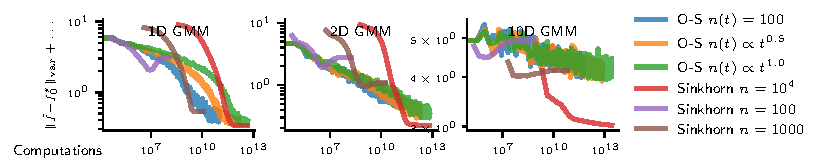
\includegraphics[width=\linewidth]{online_0.01_False_test.pdf}
    \end{widepage}
    \caption{Online Sinkhorn consistently estimate the true regularized OT potentials. Convergence here is measured in term of distance with potentials evaluated on a "test" grid of size $n=10^4$. Online-Sinkhorn can estimate potentials faster than sampling then scaling the cost matrix.}
    \label{fig:convergence}
\end{figure}

\begin{figure}[t]
    \centering
    \begin{widepage}
    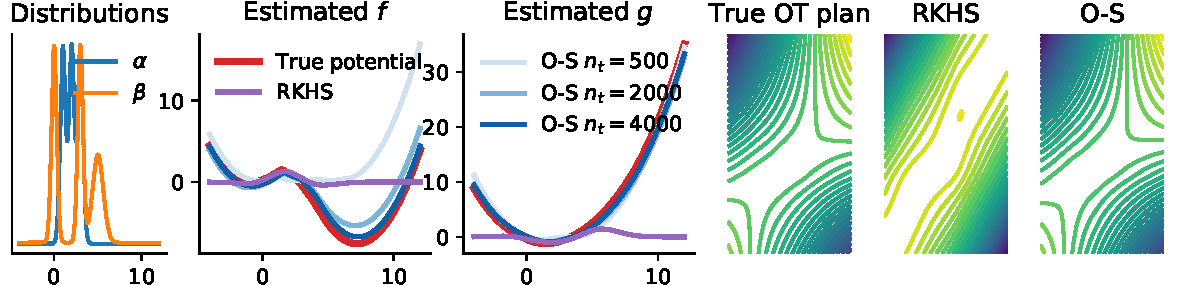
\includegraphics[width=\linewidth]{continuous.pdf}
    \end{widepage}
    \caption{Online Sinhkorn finds the correct potentials over all space, unlike SGD over a RKHS parametrization of the potentials. The plan is therefore correctly estimated everywhere.}
    \label{fig:potentials}
    \vspace{-1em}
\end{figure}

\section{Numerical experiments}\label{sec:exps}

% We have introduced and stated convergence results on the online Sinkhorn
% algorithm. These convergence results are non-quantitative and therefore
% require an experimental validation. Our experiments are three-fold: first, we
% show that online Sinkhorn correctly estimates the solutions of \eqref{eq:wass}
% and the Sinkhorn distance, overcoming the bias due to the fixed a priori
% sampling of the regular Sinkhorn algorithm. Then, we show how online Sinkhorn
% accelerates the Sinkhorn algorithm, by progressively estimating sketches of
% the dual potentials, in parallel to the computation of the distance matrix.
% Finally, we show how online Sinkhorn allows one to estimate accurately the
% geometry of the dual, significantly improving the result using SGD with RKHS
% expansions~\citep{2016-genevay-nips}.


The major purpose of online Sinkhorn (OS) is to handle OT between continuous
distributions.  We first show that it is a valid alternative to applying Sinkhorn
on a single realization of continuous distributions, using examples of Gaussian mixtures of varying dimensions.
%
We then illustrate that OS is able to estimate precisely
Kantorovich dual potentials, significantly improving the result obtained using SGD with RKHS
expansions~\citep{2016-genevay-nips}.
%
Finally, we show that OS is an efficient warmup strategy to accelerate Sinkhorn for discrete problems on several real and synthetic datasets.


% We first consider a discrete distribution $(\alpha, \beta)$, to be able to
% compute the reference distance $\Ww = \Ww(\alpha, \beta)$ and the optimal
% potentials $f^\star$, $g^\star$, using Sinkhorn algorithm. The goal here is not
% to perform better than the Sinkhorn algorithm in the long run. Indeed, the
% constraints of online Sinkhorn impose unnecessary slow-downs when dealing with
%  discrete distributions with small supports. Rather, our purpose is to illustrate the improved
% precision of online Sinkhorn for estimating true OT distances. We choose $\alpha$ and $\beta$ to be two
% discrete 1-D distributions, $\Xx=\RR$, sampled from the continuous densities
% displayed in
% \autoref{fig:potentials}. We set $\varepsilon = 10^{-2} \max_{x,y}
% C(x,y)$, where we use the squared Euclidean loss (regularized $\Ww_2$
% setting)---the distributions $\alpha$ and $\beta$ have bounded support. We use
% $\eta_t = \frac{1}{\sqrt{t}}$ for online Sinkhorn and a fixed batch-size $n$, in
% all experiments. We compare the performance of Sinkhorn, online Sinkhorn and
% random Sinkhorn, measuring $\Vert f - f^\star \Vert_{\text{var}} + \Vert g -
% g^\star \Vert_{\text{var}}$ and the absolute error $| \Ww_t - \Ww |$ versus the
% number of computations performed---the evaluation of $C(x_i, y_i)$ and the
% computation of each addition in the $C$-transform being considered as elementary
% computation units. We further report the performance of using out-of-loop
% averaging with $\gamma_t = \frac{1}{\sqrt{t}}$.

\subsection{Continuous potential estimation with online Sinkhorn}\label{sec:continuous}

\paragraph{Data and quantitative evaluation.}\label{sec:online_exp}

We measure the performance of our algorithm in a
 continuous setting, where $\alpha$ and $\beta$ are  parametric
distributions (Gaussian mixtures in 1D, 2D and 10D, with 3, 3 and 5 modes, so
that $C_{\max} \sim 1$), from which we draw samples. In the absence of reference
potentials $(f^\star, g^\star)$ (which cannot be computed in closed form),
we compute ``test'' potentials $(f^\star_0, g^\star_0)$ on realizations $\hat
\alpha_0$ and $\hat \beta_0$ of size $10000$, using Sinkhorn. We then compare
OS to Sinkhorn runs of various size , trained on realizations $N=(100,1000,
10000)$ independent of the reference grid (to avoid reducing the problem to a
discrete problem between $\hat \alpha_0$ and $\hat \beta_0$). To measure
convergence, we compute $\delta_t = \Vert \hat f_t - f^\star_0 \Vert_{\var} +           
\Vert \hat g_t -  g_0^\star \Vert_{\var}$, evaluated on the grid defined by
$\hat \alpha_0$ and $\hat \beta_0$, which constitutes a Monte-Carlo approximation of the error.
%
We evaluate OS with and without full-correction, with
different batch-size schedules (see \autoref{app:online_exp}), as well as the randomized Sinkhorn algorithm. Quantitative results are average over 5 runs. We report quantitative results for $\epsilon = 10^{-2}$ and non fully-corrective online Sinkhorn in the main text, and all other curves in Supp.~\autoref{fig:convergence_all}. In
Supp.~\autoref{fig:gaussian}, we also report results for OT between Gaussians, which is a simpler and less realistic setup, but for which closed-form expressions of the potentials are known \cite{janati_entropic_2020}.

\paragraph{Comparison to SGD.}\label{sec:compare}
%
For qualitative illustration, on the 1D and 2D problem, we consider the main existing competing
approach \citep{2016-genevay-nips}, in which $f_t(\cdot)$ is parametrized as
$\sum_{i=1}^{n_t} \alpha_t \kappa(\cdot, x_i)$ (and similarly for $g_t$), where
$\kappa$ is a reproducing kernel (typically a Gaussian). This differs
significantly from online Sinkhorn, where we express $e^{-f_t}$ as a Gaussian
mixture. The dual problem \eqref{eq:sinkhorn} is solved using SGD, with convergence guarantees on the dual energy.  As advocated
by the authors, we run a grid search over the bandwidth parameter~$\sigma$ of
the Gaussian kernel to select the best performing runs.


\paragraph{Earlier potential convergence.}
We study convergence curves in \autoref{fig:convergence}, comparing algorithms
at equal number of multiplications. OS outperforms or matches Sinkhorn for $N=100$
and $N=1000$ on the three problems; it approximately matches the performance of
Sinkhorn on $N=10000$ new iterates on the 1D and 2D problems. On the two
low-dimensional problems, online Sinkhorn converges faster than Sinkhorn at the
beginning. Indeed, it initiates the computation of the potentials early, while the Sinkhorn
algorithm must wait for the cost matrix to be filled. This leads us
to study online Sinkhorn as a catalyser of Sinkhorn in the next paragraph. OS
convergence is slower (but is still noticeable) for the higher dimensional problem.
Fully-corrective OS performs better in this case (see Supp.~\autoref{fig:convergence_refit}). We also note that randomized Sinkhorn with batch-size $N$ performs on par with Sinkhorn of size $N$ (Supp.~\autoref{fig:convergence_randomized}).

\paragraph{Better-extrapolated potentials.} As illustrated in
\autoref{fig:potentials}, in 1D, online Sinkhorn refines the potentials $(\hat f_t, \hat g_t)_t$
until convergence toward $(f^\star, g^\star)$. Supp. \autoref{fig:potentials_2d} shows a visualisation for 2D GMM. As the parametrization~\eqref{eq:param} is
adapted to the dual problem, the algorithm quickly identifies the correct shape of
the optimal potentials---as predicted by \autoref{prop:convergence_true}. In
particular, OS estimates potentials with much less errors than SGD in a RKHS in
areas where the mass of $\alpha$ and $\beta$ is low. This allows to consistently estimate the transport plan, which cannot be achieved using SGD. SGD did not converge for $\epsilon < 10^{-1}$, while online Sinkhorn remains stable. OS does not require to set a bandwidth.

\setlength{\tabcolsep}{2pt}

\begin{figure}[t]
    \begin{widepage}
    \begin{minipage}{.7\linewidth}
    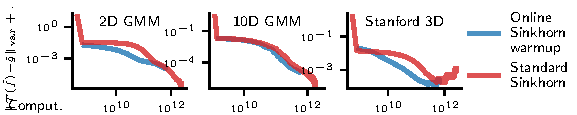
\includegraphics[width=\linewidth]{online+full_0.001_err.pdf}
    \end{minipage}%
    \hfill
    \begin{minipage}{.3\linewidth}
        \centering
        \small
        \begin{tabular}{lrrrr}
            \toprule
            $- \log \varepsilon$
            &  4 & 3 & 2 & 1 \\
            \midrule
            Stanford      &     5.3x &    4.4x &    2.3x &    1.2x \\
            10D GMM     &     1.4x &    1.5x &    1.3x &    1.2x \\
            2D GMM      &    17x &    3.7x &    1.3x &    2.0x \\
            \bottomrule
            \end{tabular}
    \end{minipage}
    \end{widepage}
    \stepcounter{table}
    \caption{Online Sinkhorn allows to warmup Sinkhorn during the evaluation of the cost matrix, and to speed discrete optimal transport. Table \thetable: Speed-ups provided by OS vs S to reach a $10^{-3}$ precision.}
    \label{fig:warmup}
    \vspace{-.8em}
\end{figure}


\subsection{Accelerating Sinkhorn with online Sinkhorn warmup}\label{sec:accelerating}

The discrete Sinkhorn algorithm requires to compute the full cost matrix $\Cz
\eqdef (C(x_i,y_i))_{i,j}$  of size $N \times N$, prior to estimating the
potentials $\f_1 \in \RR^N$ and $\g_1 \in \RR^N$ by a first $C$-transform. In
contrast, online Sinkhorn can progressively compute this matrix while computing
first sketches of the potentials. The extra cost of estimating the initial
potentials without full-correction is simply $2 N^2$, i.e. similar to filling-up
$\Cz$. We therefore assess the performance of \textit{online Sinkhorn as
Sinkhorn warmup} in a discrete setting. Online Sinkhorn is run with batch-size
$n$ during the first iterations, until observing each sample of $[1,N]$, i.e.
until the cost matrix $\Cz$ is completely evaluated. From then, the subsequent
potentials are obtained using full Sinkhorn updates. We consider the GMMs of
\autoref{sec:continuous}, as well as a 3D dragon from Stanford 3D scans
\cite{turk1994zippered} and a sphere of size $N=12000$. We measure convergence
using the error $\Vert \Ctrans{\hat f_t}{\alpha} - \hat g_t
\Vert_{\var} + \Vert \Ctrans{\hat g_t}{\beta} - \hat f_t \Vert_{\var}$,
evaluated on the support of $\alpha$ and $\beta$; this error goes to $0$. We use
$n(t) = \frac{N}{100} (1+0.1t)^{1/2}$---results vary little with the exponent.


\paragraph{Results.} We report convergence curves for $\varepsilon = 10^{-3}$ in
\autoref{fig:warmup}, and speed-ups due to OS in Table 1. Convergence curves for
different $\varepsilon$ are reported in Supp.~\autoref{fig:warmup_full}. The
proposed scheme provides an improvement upon the standard Sinkhorn algorithm.
After $N^2 d$ computations (the cost of estimating the full matrix $C$), both
the function value and distance to optimum are lower using OS: the full Sinkhorn
updates then relay the online updates, using an accurate initialization of the
potentials. The \textit{OS warmed-up} Sinkhorn algorithm then maintains its
advantage over the standard Sinkhorn algorithm during the remaining iterations.
The speed gain increases as $\varepsilon$ reduces and the OT problem becomes
more challenging. Sampling without replacement brings an additional speed-up.
